\documentclass{article}

\usepackage[a4paper]{geometry}
\usepackage[spanish]{babel}
\usepackage{xcolor}

\usepackage{mathbbol}
\usepackage{amsmath}
\usepackage{amsfonts}
\usepackage{hyperref}
\usepackage{graphicx}

% Cambiar 'Cuadro' -> 'Tabla'
\addto\captionsspanish{
    \renewcommand{\tablename}{Tabla}
}

\begin{document}

\begin{center}
    {\Large Aprendizaje Automático para Datos en Grafos} \\
    {\LARGE \textbf{Laboratorio 1}} \\
    \vspace{2em}
    \begin{minipage}{0.45\textwidth}
        \centering
        Graciana Castro \\
        4.808.848-2 \\
        gcastro@fing.edu.uy
    \end{minipage}
    \hfill
    \begin{minipage}{0.45\textwidth}
        \centering
        Julian O'Flaherty \\
        6.285.986-9 \\
        julian.o.flaherty@fing.edu.uy
    \end{minipage}
\end{center}


\section{Introducción}
Se presenta a continuación el informe del Laboratorio 1 para la materia Aprendizaje Automático para Datos en Grafos. Tiene como objetivo principal afianzar los conocimientos dados en el teórico sobre descriptores del grafo (por ejemplo: cantidad de nodos, cantidad de aristas, cantidad de aristas dirigidas) y distintas medidas de centralidad para identificar nodos y relaciones importantes entre ellos. Además, se busca familiarizarnos con las bibliotecas \textit{NetworkX} y \textit{Pytorch Geometric}, dos bibliotecas de Python utilizadas para trabajar con datos en grafos.

El laboratorio se separa en dos ejercicios. En el primero se trabaja con la base de datos \textit{Enron Scandal} \footnote{\url{https://www.cs.cmu.edu/~enron/}} mientras que para el segundo se utiliza la base \textit{Zachary's Karate Club}. El informe se divide en la sección \ref{sec: ej1} donde se presenta el Ejercicio 1 y la sección \ref{sec: ej2} para el Ejercicio 2. En cada una se describe la base de datos utilizada, resultados obtenidos y conclusiones. Se puede consultar el código implementado en el repositorio de GitHub \url{https://github.com/j-oflaherty/AA-grafos/blob/main/lab1/Lab1_AAG2025.ipynb}.

\section{Ejercicio 1} \label{sec: ej1}
En este ejercicio se trabaja con la base de datos \textit{Enron Scandal}, que contiene correos electrónicos de empleados de la empresa Enron. Se hizo pública después del escándalo financiero de la empresa a principios de los 2000s. Se encuentra estructurada como un grafo dirigido, donde los nodos del grafo representan a los empleados y las aristas dirigidas representan los correos electrónicos enviados entre ellos.

Para este trabajo, se descarta el cuerpo de los correos electrónicos, quedando solo los datos de cual nodo interactuó con cual y el nombre de cada nodo. Además, se realizó una tarea previa de limpieza eliminando los \textit{self-loops} (aristas que tienen igual nodo de entrada y de salida).


\subsection{Análisis del grafo completo}
En primera instancia se trabaja con el grafo que considera todos los correos electrónicos intercambiados entre los empleados. El grafo resultante se muestra en la figura \ref{fig:grafo}, donde como dice el título, el grosor de la arista está determinado por la cantidad de correos intercambiados entre los dos nodos y el color del nodo está determinado por su \textit{betweeness centrality}, que mide la importancia de un nodo al pasaje de información. Se pueden observar nodos que no tienen ninguna arista entrante ni saliente, como ser el 117, que son empleados que se encontraban en la base de datos debido a que se autoenviaron correos pero no recibieron ni enviaron otros.

\begin{figure}[htb]
    \centering
    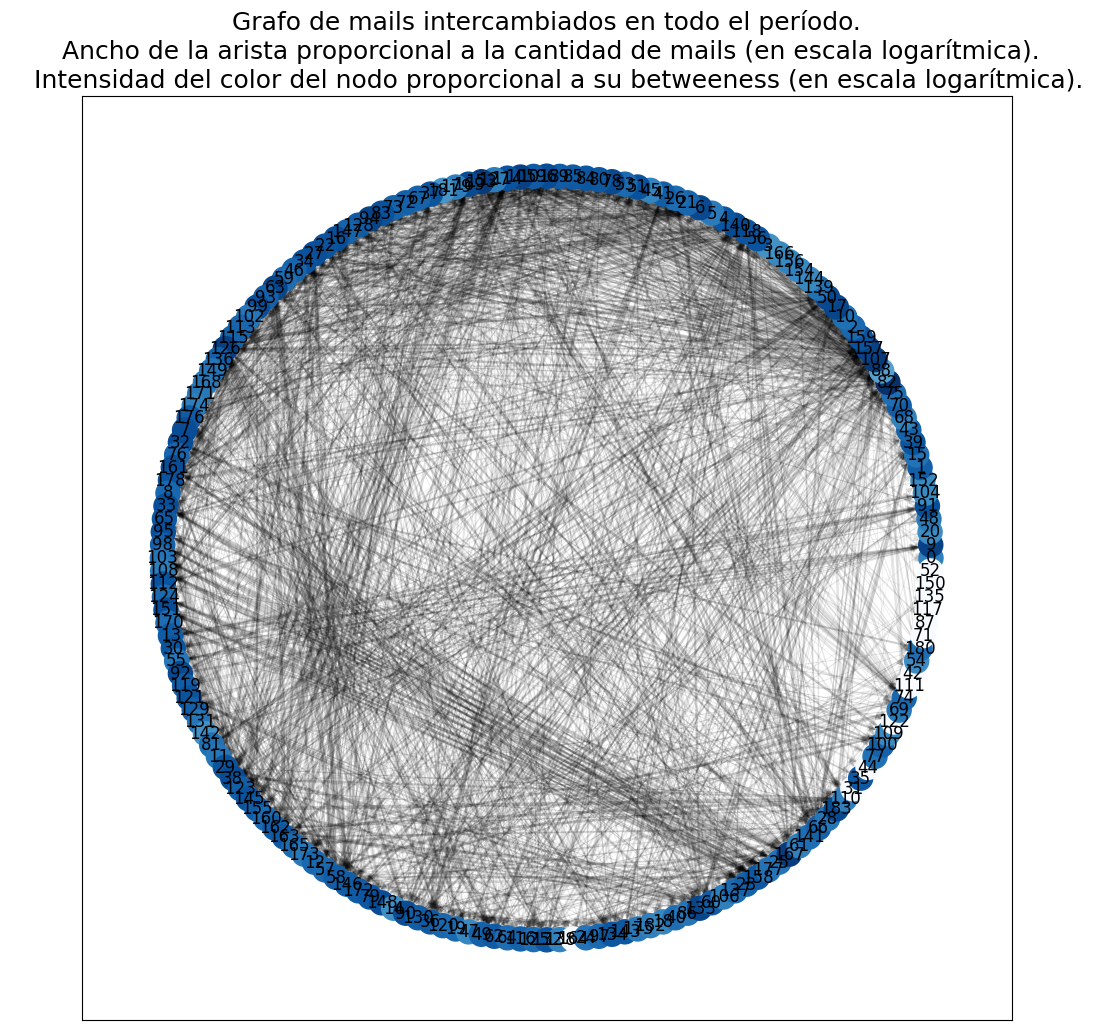
\includegraphics[width=0.8\linewidth]{imagenes/ej1/grafo.png}
    \caption{Esquema del grafo de correos electrónicos de Enron.}
    \label{fig:grafo}
\end{figure}

Este grafo tiene en total 184 nodos conectados por 3007 aristas dirigidas (valores obtenidos a partir de las funciones \verb|number_of_nodes| y \verb|number_of_edges| de \textit{NetworkX}). Para calcular la cantidad de aristas no dirigidas, primero convertimos el grafo en uno no dirigido (con la función \verb|to_undirected|) y luego volvimos a utilizar la función \verb|number_of_edges|. De esta forma, se obtuvo que el grafo tiene 2097 aristas no dirigidas, lo que indica que gran parte de los intercambios de mails son unilaterales. Se valida esto al calcular los arcos mutuos, donde obtenemos que 910 los pares de nodos intercambiaron mails de ida y vuelta. Para calcular esto, se pasa el grafo a un grafo dirigido en el que se consideran solo los arcos mutuos (utilizando el parámetro \verb|reciprocal=True| de la misma función \verb|to_undirected|). Otra forma de calcularlo es haciendo la resta entre el total de aristas dirigidas y el total de aristas no dirigidas, ya que esta diferencia indica la cantidad de aristas que no se cuentan porque ya fue contada la arista en sentido contrario.

Para el cálculo del grado de entrada y de salida se puede utilizar las funciones \verb|in_degree| y \verb|out_degree| de \textit{NetworkX} o realizar el cálculo de aristas de entrada y salida a partir de la matriz de adyacencia. Se tienen tres nodos con grado de entrada cero, dos de los cuales además tienen grado de salida igual a cero. Son nodos aislados de la red, que representan empleados que se auto enviaron correos (como fue mencionado antes, las aristas asociadas fueron descartadas en el preprocesado).

Se muestran a continuación las tablas obtenidas al observar los nodos con grado de entrada y salida cero (tablas \ref{tab:in_zero} y \ref{tab:out_zero} respectivamente).

\begin{table}[htb]
    \centering
    \begin{tabular}{|c|c|r|}
        \hline
        \textbf{Nodo} & \textbf{mail} & \textbf{name and more}            \\
        \hline
        71            & j..kaminski   & Vince Kaminski Manager Risk Ma... \\
        117           & mary.fischer  & Mary Fischer Employee             \\
        135           & m..smith      & xxx                               \\
        \hline
    \end{tabular}
    \caption{Tabla de nodos con grado de entrada cero.}
    \label{tab:in_zero}
\end{table}

% \begin{figure}[htb]
%     \centering
%     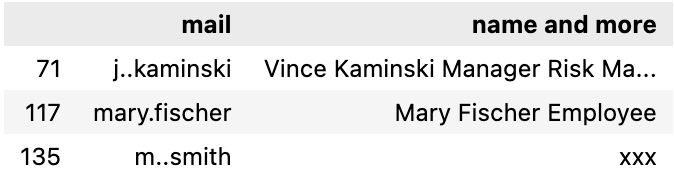
\includegraphics[width=0.6\linewidth]{imagenes/ej1/in_degree_zero.png}
%     \caption{Tabla de nodos con grado de entrada cero.}
%     \label{fig:in_zero}
% \end{figure}

\begin{table}[htb]
    \centering
    \begin{tabular}{|c|c|r|}
        \hline
        \textbf{Nodo} & \textbf{mail}   & \textbf{name and more}                  \\
        \hline
        164           & steven.south    & xxx                                     \\
        122           & michele.lokay   & Michelle Lokay Employee Admi...         \\
        111           & mark.e.haedicke & Mark Haedicke Managing Director Lega... \\
        42            & e.taylor        & Mark Taylor Employee                    \\
        71            & j..kaminski     & Vince Kaminski Manager Risk Ma...       \\
        87            & judy.hernandez  & xxx                                     \\
        117           & mary.fischer    & Mary Fischer Employee                   \\
        150           & rob.gay         & xxx                                     \\
        52            & gretel.smith    & xxx                                     \\
        \hline
    \end{tabular}
    \caption{Tabla de nodos con grado de salida cero.}
    \label{tab:out_zero}
\end{table}

% \begin{figure}[htb]
%     \centering
%     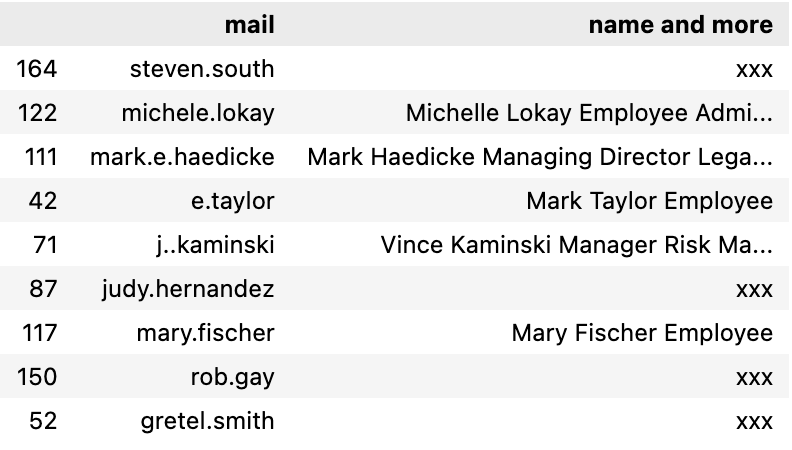
\includegraphics[width=0.6\linewidth]{imagenes/ej1/out_degree_zero.png}
%     \caption{Tabla de nodos con grado de salida cero.}
%     \label{fig:out_zero}
% \end{figure}

\subsection{Análisis de empleados populares}
Se consideran empleados populares aquellos que recibieron correos de más de 30 personas distintas o enviaron correos a más de 30 personas distintas. Se muestra en la figura \ref{fig:grafos_populares} los grafos completos con los empleados populares marcados en rojo.

\begin{figure}[htb]
    \centering
    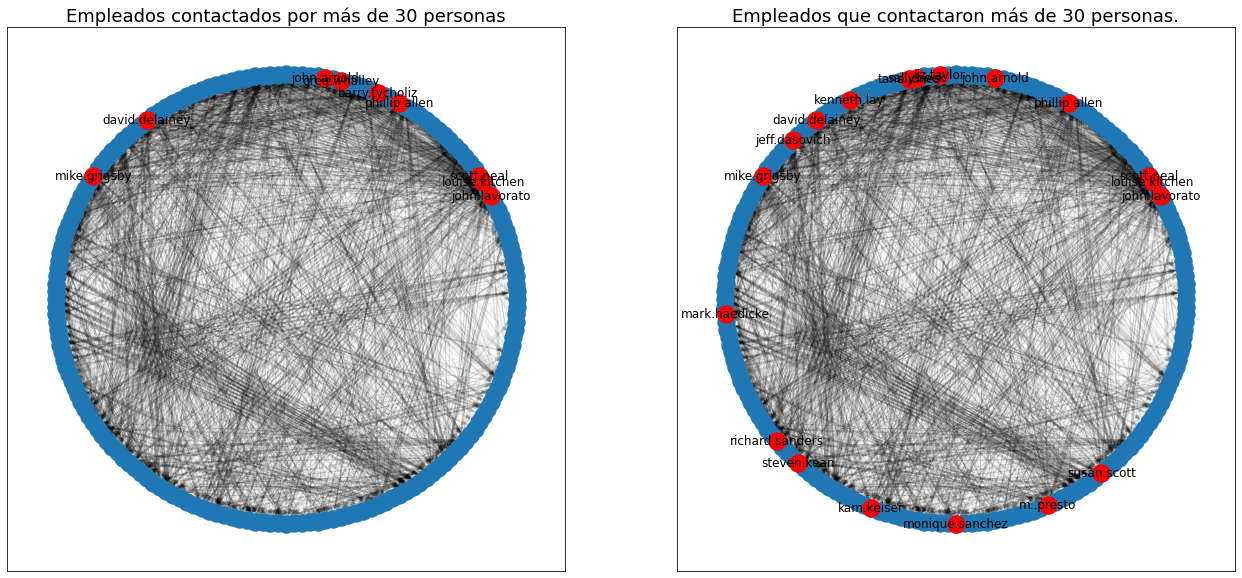
\includegraphics[width=0.8\linewidth]{imagenes/ej1/empleados_populares.png}
    \caption{Grafo de correos electrónicos de empleados populares.}
    \label{fig:grafos_populares}
\end{figure}

Se puede observar que los empleados populares tienden a estar más conectados dentro de la red, lo que sugiere que tienen un papel más central en la comunicación de la empresa. También se observa que varios de los empleados se encuentran destacados en los dos grafos, lo que indica que son tanto receptores como emisores activos. Si se busca en la base de datos quienes son estos empleados, se encuentran varios nombres reconocidos, como por ejemplo \textit{Jeff Skilling} (ex CEO de Enron), \textit{Kenneth Lay} (ex presidente de Enron) y \textit{Andrew Fastow} (ex CFO de Enron). En la columna \textit{name and more}, que en muchos casos muestra el nombre y puesto de la empresa, se observan varios individuos con la etiqueta \textit{CEO}, \textit{President} y \textit{Vice President}.

\subsection{Histograma de grados de los nodos}

La figura \ref{fig:histogramas_grados} muestra la distribución de los grados de entrada y salida. Se observa que la mayoría de los nodos tienen grados de entrada y salida bajos, lo que indica que la mayoría de los empleados envían y reciben correos con pocos otros empleados. El grado de entrada está más concentrado entre 5 y 25, con pocos nodos que reciben correos de muchas personas.

Por otro lado, la distribución del grado de salida presenta una cola más larga: existen algunos nodos que envían correos a muchos destinatarios (hasta cerca de 100), lo que podría indicar roles administrativos o de coordinación, que suelen enviar comunicaciones generales para todos los empleados. En general, la distribución es asimétrica, especialmente en el grado de salida, lo que sugiere que hay nodos con comportamiento muy diferente al promedio. Esto indica que el grafo tiene una estructura donde la mayoría de los nodos interactúan con pocos otros, pero existen algunos nodos con alta actividad de envío, posiblemente personas con roles clave en la comunicación interna.

\begin{figure}[htb]
    \centering
    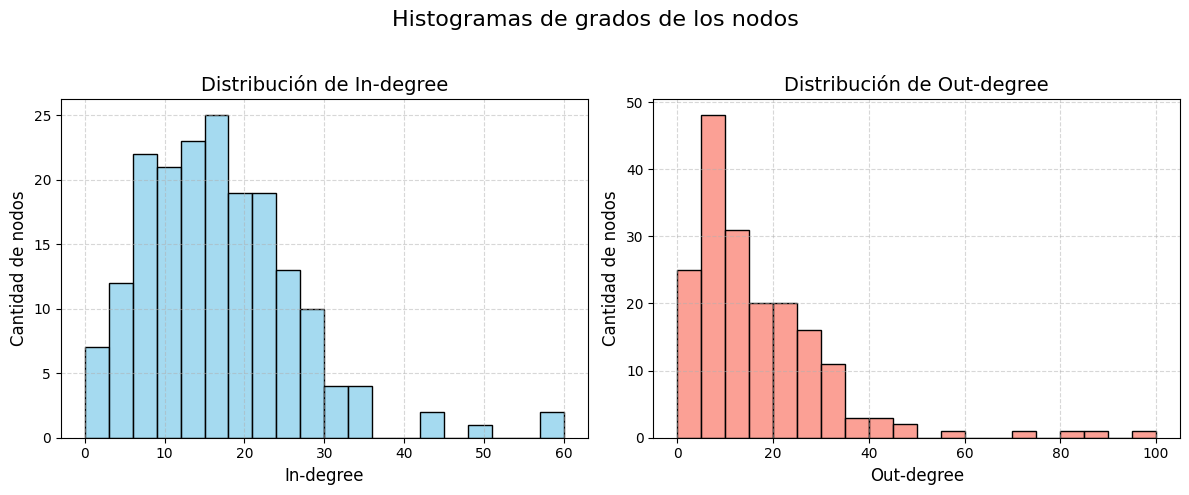
\includegraphics[width=0.8\linewidth]{imagenes/ej1/histogramas_grados_nodos.png}
    \caption{Histograma de grados de los nodos.}
    \label{fig:histogramas_grados}
\end{figure}

\subsection{Análisis temporal del grafo}
% completar
Los datos cuentan con etiquetas temporales, por lo que podemos analizar la evolución del grafo y su estructura a lo largo del tiempo. El primer paso consiste en
agrupar los datos semanalmente y generar el grafo de interacciones asociado a esa semana.  El modelado temporal nos permite hacer un análisis de comportamientos
anómalos en el funcionamiento de la empresa, lo que puede indicar eventos del escándalo.

\subsubsection{Indicadores de nodos}

Los indicadores de nodo son métricas que evalúan alguna característica del nodo respecto al grafo. En nuestro caso, vamos a tomar la \emph{Betweeness Centrality} y el \emph{PageRank} como indicadores. \emph{Betweeness Centrality}, mide la importancia de un nodo al pasaje de la información, y se define como:
\begin{equation}
    c(v) = \sum_{s \neq v \neq t} \frac{\sigma_{st}(v)}{\sigma_{st}}
    \label{eq:betweeness_centrality}
\end{equation}
Donde:
\begin{itemize}
    \item $\sigma_{st}(v)$: número de caminos más cortos que pasan por $v$ entre $s$ y $t$
    \item $\sigma_{st}$: número total de caminos más cortos entre $s$ y $t$
\end{itemize}
\emph{PageRank}, por su parte, es una métrica que evalúa la importancia de un nodo en el grafo en base a su relación con nodos importantes. Esta se define como:
\begin{equation}
    PR(v) = (I - \alpha A^\top D^{-1})^{-1} \mathbf{1}
    \label{eq:page_rank}
\end{equation}
Donde:
\begin{itemize}
    \item $A$: matriz de adyacencia del grafo
    \item $D$: matriz de grados del grafo
    \item $\alpha$: factor de amortiguación, tipicamente $0.85$ (valor default de \textit{NetworkX})
\end{itemize}

Para medir la evolución temporal de los indicadores, se calculan los indicadores para cada subgrafo semanal y se toma el máximo valor y el nodo al que corresponde.

\begin{figure}[htb]
    \centering
    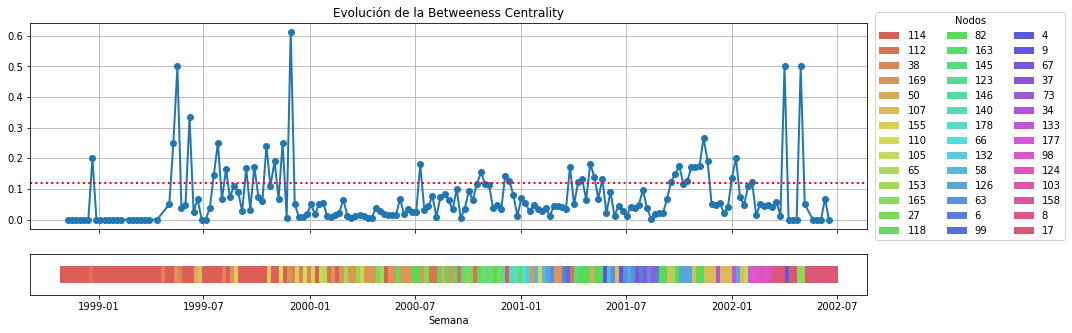
\includegraphics[width=\linewidth]{imagenes/ej1/betweeness.png}
    \caption{Evolución de la Betweeness Centrality. La linea roja punteada es el valor máximo del grafo completo.}
    \label{fig:betweeness_centrality}
\end{figure}

\begin{figure}[htb]
    \centering
    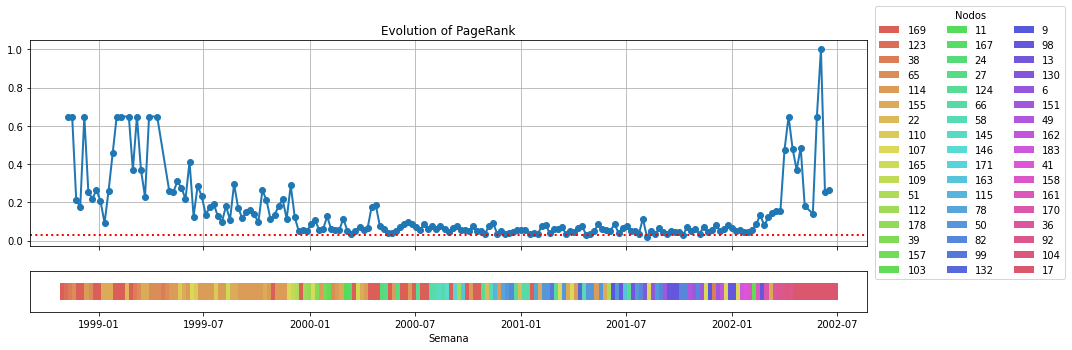
\includegraphics[width=\linewidth]{imagenes/ej1/pagerank.png}
    \caption{Evolución de la PageRank. La linea roja punteada es el valor máximo del grafo completo.}
    \label{fig:page_rank}
\end{figure}

En la figura \ref{fig:betweeness_centrality} se observa la evolución temporal de la \textit{Betweeness Centrality}. Una primera observación es que al principio y al final del periodo, se obtienen valores muy bajos porque los grafos tienen pocos nodos, dado que son semanas de poca actividad.
Debido a la variedad de nodos que toman el valor máximo semana a semana, la representación visual se torna dificil, pero aún así se puede notar como nodos que incialmente no eran relevantes toman relevancia a medida que pasa el tiempo. Estas mismas observaciones aplican a la figura \ref{fig:page_rank}\footnote{Los colores son independientes entre las dos figuras.}, solo que al principio y al final del periodo se obtienen valores más altos por la naturaleza de la métrica.

En la figura~\ref{fig:betweeness_centrality}, el pico más alto coincide con un evento de la controversia, el lanzamiento de \emph{Enron Online}. Hay un segundo pico alrededor de Julio del 2000 que coincide con la \emph{EBS Blockbuster Parnership}. Cerca de Enero 2002 observamos nuevos picos, que coincide con las fechas donde \emph{Enron} se declara en bancarrota.

Del análisis de la figura~\ref{fig:page_rank} es más dificil detectar eventos puntuales, pero se nota como el comportamiento durante la controversia pareciera ser anómalo respecto a las semanas previas y posteriores, donde hubo mucho más movimiento en la red que lo normal.

\subsubsection{Indicadores de grafo}

Se puede realizar también un análisis de métricas a nivel del grafo entero. Estas métricas evalúan el comportamiento de la red en su totalidad en vez del comportamiento individual de los nodos.

Para este análisis, se eligieron 5 métricas:
\begin{itemize}
    \item \emph{Número de nodos}: Número de nodos del grafo. Indica la cantidad de personas involucradas en la red cada semana.
    \item \emph{Número de aristas}: Número de aristas del grafo. Indica el nivel de interacción entre las personas en la red cada semana.
    \item \emph{Grado máximo}: Grado máximo de los nodos del grafo. Indica si las interacciones se dan entre muchas personas, o si fueron entre grupos más chicos de personas.
    \item \emph{Grado promedio}: Promedio de los grados de los nodos del grafo. Indica el nivel de interacción promedio entre las personas en la red cada semana.
    \item \emph{Coeficiente de agrupamiento promedio}: Promedio de los coeficientes de agrupamiento de los nodos del grafo. Indica si las interacciones se dieron entre grupos de personas, o si fueron entre personas individuales.
\end{itemize}

\begin{figure}[htb]
    \centering
    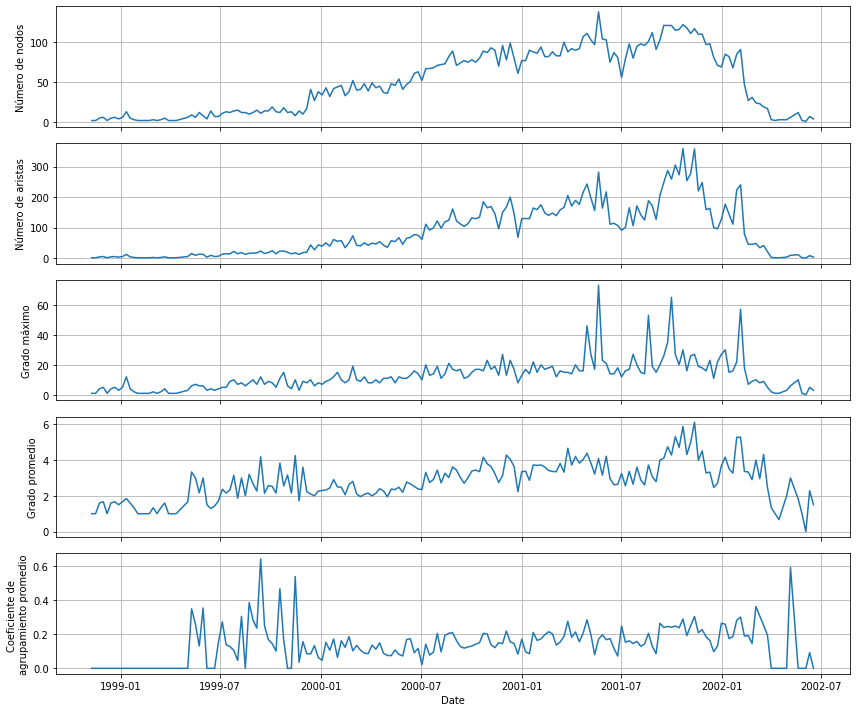
\includegraphics[width=\linewidth]{imagenes/ej1/metricas_grafo.png}
    \caption{Evolución de las métricas del grafo.}
    \label{fig:metricas_grafo}
\end{figure}

En la figura~\ref{fig:metricas_grafo} se observa la evolución temporal de las métricas del grafo. Se puede observar que el número de nodos y el número de aristas aumentan a lo largo del tiempo, lo que indica que la cantidad de involucrados y la cantidad de interacciones va creciendo a lo largo que se desarrolla la controversia.

El grado promedio sigue la misma tendencia, mientras que el grado máximo tiene picos marcados sobre el final del periodo. El coeficiente de agrupamiento promedio es el más erratico, con muchos picos al principio y sobre el final del periodo.

Al igual que con los indicadores de nodos, podemos ver picos en el coeficiente de agrupamiento promedio cerca de diciembre del 1999, que coincide con el lanzamiento de \emph{Enron Online}. Otra fecha notable, donde todas las gráficas presentan un pico, es a inicios del 2001, cuando Stephen Cooper como \emph{CEO}. Otro evento detectable es el pico que se da en el grado máximo un poco antes de Julio 2001, que coincide con una reunión de Cuatrimestre.

\section{Ejercicio 2} \label{sec: ej2}
En este ejercicio se trabaja con la base de datos \textit{Zachary's Karate Club}, que contiene las interacciones entre los miembros de un club de karate. Representa las relaciones de amistad entre los miembros de un club de karate universitario, estudiadas por Wayne Zachary en la década de 1970. El grafo contiene 34 nodos (miembros) que representan a los miembros del club y las aristas son no dirigidas y sin pesos e indican la existencia de una relación social fuera del club.

Se trabaja principalmente con la biblioteca \textit{Pytorch Geometric}, con el objetivo de familiarizarse con el manejo de grafos en esta biblioteca y realizar análisis sobre la estructura del grafo. El objetivo del ejercicio es verificar empíricamente con funcionalidades de \textit{Pytorch Geometric} las propiedades de la matriz Laplaciana que se demuestran en la subsección \ref{subsec:opcional}.

\subsection{Vectores y valores propios de la Matriz Laplaciana}
Para calcular la matriz Laplaciana del grafo, se emplea la función \verb|get_laplacian| de \textit{Pytorch Geometric}. Posteriormente, se obtienen los vectores y valores propios utilizando \verb|torch.linalg.eig| y \verb|torch.linalg.eigvalsh|. Como resultado, se observa que uno de los valores propios es $8.61 \times 10^{-7}$, valor prácticamente nulo, lo que confirma la propiedad teórica de que un valor propio es cero.

Ahora que sabemos que cero es valor propio, se puede verificar que el vector de 1s es vector propio asociado, utilizando que $Ax = \lambda x$. En este caso, $A$ es la matriz Laplaciana $L$ y $x$ es el vector de 1s. El producto de $L \cdot \mathbf{1}$ da como resultado el vector nulo, confirmando que $\mathbf{1}$ es efectivamente un vector propio asociado al valor propio cero.

A partir del cálculo de los valores propios de la matriz Laplaciana, se observa que todos los valores propios son no negativos, lo que confirma que la matriz es semidefinida positiva. El valor propio más pequeño es cero, y los demás valores propios son positivos.

\subsection{Matriz de Incidencia}
Utilizando la funcion de \textit{Pytorch Geometric} \verb|get_incidence|, se puede obtener la matriz de incidencia del grafo. Luego, simplemente realizando el producto de la matriz de incidencia por su traspuesta, se puede verificar fácilmente que el resultado es igual a la matriz Laplaciana.

\subsection{Ejercicio opcional} \label{subsec:opcional}

En esta sección se demuestran algunas propiedades de la matriz Laplaciana.

\newcommand{\ones}[1]{\mathbb{1}_{#1}}
\newcommand{\lap}{\mathbf{L}}
\newcommand{\diag}{\mathbf{D}}
\newcommand{\adj}{\mathbf{A}}
\newcommand{\bm}{\tilde{\mathbf{B}}}
\newcommand{\x}{\mathbf{x}}

Sea $G(V,E)$ un grafo simple (no dirigido, sin pesos y sin auto-aristas), con cantidad de vértices $N_v = |V|$ y cantidad de aristas $N_e = |E|$, y matriz de adyacencia $\mathbf{A}$. Sea $\mathbf{D} = \text{diag}(d_{1},\dots, d_{N_v})$ la matriz de grados y $\mathbf{L}=\mathbf{D}- \mathbf{A}$ la matriz laplaciana de $G$.

\subsubsection{Vector propio $\ones{N_v}$}
\label{subsec:vector_propio_1}

Verificaremos que $\ones{N_v}$ es vector propio de $\lap$ con valor 0. Desarrollemos la multiplicación:

\begin{equation}
    \lap \cdot \ones{N_v} = (\diag - \adj) \cdot \ones{N_v}  = \diag \cdot \ones{N_v} - \adj \cdot \ones{N_v} \stackrel{(a)}{=} \vec{0}
    \label{eq:1_vecpropio_L}
\end{equation}

Donde en (a) se usa que $\adj \cdot \ones{N_v} = [d_1, \dots, d_{N_v}]$, resultado que
se obtiene trivialmente a partir de la definición de matriz de adyacencia.
Por lo tanto, \eqref{eq:1_vecpropio_L} prueba que $\ones{N_v}$ es vector propio de $\lap$ con valor 0.

\subsubsection{Relación del laplaciano y la matriz de incidencia}

Aunque $G$ es un grafo no dirigido, podemos asignarle a cada arista en $E$ una orientación ``virtual'' arbitraria: para cada arista elegimos arbitrariamente uno de sus vértices como nodo inicial y el otro como nodo final. Dada esa asignación, definimos la \textbf{matriz de incidencia signada} $\bm \in \{-1,0,1\}^{N_v\times N_e}$ con entrada $i,e$ dada por:
\begin{equation}
    \bm_{ie} = \left\lbrace
    \begin{array}{r l}
        1,  & \text{si el vértice } i \text{ es el nodo inicial de la arista } e \\
        -1, & \text{si el vértice } i \text{ es el nodo final de la arista } e   \\
        0,  & \text{en otro caso}
    \end{array}
    \right. .
    \label{eq:matrix_incidencia}
\end{equation}

Demostraremos que la matriz laplaciana puede descomponerse como $\mathbf{L}=\tilde{\mathbf{B}}\tilde{\mathbf{B}}^\top$. Comencemos analizando el producto de $\bm\cdot\bm^\top$.

Para la diagonal:
\begin{equation}
    \label{eq:BB_ii}
    \bm\bm^\top_{ii} = \bm_i \cdot \bm_i^\top = \sum_{e\in E} \bm_{ie}^2 = d_i
\end{equation}

Para los valores fuera de la diagonal:
\begin{equation}
    \label{eq:BB_ij}
    \bm\bm^\top_{ij} = \bm_i\cdot\bm_j^\top = \sum_{e\in E} \bm_{ie} * \bm_{je} = \left\lbrace
    \begin{array}{r l}
        -1, & \text{si $\exists e\in E$ entre i y j}         \\
        0,  & \text{si $!\exists e \in E$ que conecte i y j}
    \end{array}
    \right.
\end{equation}
donde la última igualdad sucede porque solo hay una arista en $e \in E$ donde
$\bm_{ie}$ y $\bm_{je}$ son ambos no nulos, y para esa arista se cumple que uno es
$1$ y el otro $-1$. Uniendo los resultados de \eqref{eq:BB_ii} y \eqref{eq:BB_ij} obtenemos:

\begin{equation}
    \label{eq:L_igual_BB}
    \bm\bm^\top_{ij} = \left\lbrace
    \begin{array}{r l}
        d_i, & \text{si $i=j$}                                        \\
        -1,  & \text{si $i\neq j$ y existe una arista entre i y j}    \\
        0,   & \text{si $i\neq j$ y no existe una arista entre i y j}
    \end{array}
    \right. = \lap
\end{equation}
que coincide con la definición del laplaciano.

\subsubsection{$\lap$ simétrica y semidefinida positiva}

La demostración de $\lap$ simétrica surge fácilmente aplicando propiedades de la traspuesta. Partiendo del resultado \eqref{eq:L_igual_BB}:
\begin{equation}
    \lap^\top = (\bm\bm^\top)^\top = (\bm^\top)^\top \bm^\top = \bm\bm^\top = \lap
\end{equation}

Para demostrar que es semidefinida positiva, tomemos un vector $\x = [x_1, x_2, \dots, x_{N_v}]^\top \in \mathbb{R}^{N_v}$
cualquiera y calculemos $\x^\top\lap\x$.
\begin{equation*}
    \x^\top\lap\x = \x^\top \bm\bm^T\x = (\x^\top\bm)(\x^\top\bm)^\top
\end{equation*}
De la definición \eqref{eq:matrix_incidencia} de la matriz de incidencia, es trivial que $\x^\top \bm$ es un vector de dimensión $N_e$, donde el k-esimo valor es $x_i-x_j$ con $(i,j) = e_k \in E$.  Por lo tanto:
\begin{equation}
    \x^\top\lap\x = (\x^\top\bm)(\x^\top\bm)^\top = \sum_{(i,j)\in E} (x_i-x_j)^2 \geq 0
\end{equation}
quedando demostrado que $\lap$ es semidefinida positiva.

\subsubsection{Grafo G no conexo}

Si el grafo G es no conexo, podemos pensarlo como $N_c$ subgrafos conexos. De esa forma
obtenemos $N_c$ conjuntos de nodos $V_i$, aristas $E_i$, matrices de adyacencia $\adj_i$ y matrices de grado $\diag_i$. Con este modelado, es trivial ver que las matrices de adyacencia y de grados quedan:
\begin{equation*}
    \begin{array}{l c r}
        \adj = \left(\begin{matrix}
                             \adj_1 & 0      & \dots  & 0          \\
                             0      & \adj_2 & \dots  & 0          \\
                             \vdots & \vdots & \ddots & \vdots     \\
                             0      & 0      & \dots  & \adj_{N_c}
                         \end{matrix}\right)
         &  &
        \diag =\left(\begin{matrix}
                             \diag_1 & 0       & \dots  & 0           \\
                             0       & \diag_2 & \dots  & 0           \\
                             \vdots  & \vdots  & \ddots & \vdots      \\
                             0       & 0       & \dots  & \diag_{N_c}
                         \end{matrix}\right)
    \end{array}
\end{equation*}
Como el laplaciano cumple que $\lap = \diag - \adj$, y ambas matrices son diagonale por bloques, el laplaciano es diagonal por bloques.

Partiendo del resultado obtenido en la sección~\ref{subsec:vector_propio_1}, concluimos que tenemos $N_c$ vectores propios con valor 0. Cada bloque del laplaciano tiene vector propio con valor 0 al vector con unos en la entradas asociadas al bloque y 0 en el resto de entradas, lo que resulta en $N_c$ vectores ortogonales tal que $\lap \mathbf{v} = \vec{0}$.

\end{document}